\documentclass{beamer}
\usepackage[utf8]{inputenc}

\usetheme{Madrid}
\usecolortheme{default}

\usepackage{amsmath, amsfonts, amssymb, graphicx, geometry, lipsum}
\usepackage{hyperref}
\usepackage{indentfirst}
\usepackage[all,cmtip]{xy}
\usepackage{float}
\usepackage[numbers,square]{natbib}

\newcommand{\N}{\mathbb{N}}
\newcommand{\Z}{\mathbb{Z}}
\newcommand{\Q}{\mathbb{Q}}
\newcommand{\R}{\mathbb{R}}
\newcommand{\C}{\mathbb{C}}
\newcommand{\F}{\mathbb{F}}
\newcommand{\PP}{\mathbb{P}}
\newcommand{\HH}{\mathbb{H}}
\newcommand{\norm}[1]{\left\lVert #1 \right\rVert}
\newcommand{\innerp}[2]{\langle #1, #2 \rangle}

\DeclareMathOperator{\di}{d\!}

\title[Dynamical Systems of Particles]{Dynamical Systems of Particles\\ Around a Kerr Black Hole\\
{\small University of Toronto}}
\author{Haocheng Sun}
\date{Winter 2025}

\begin{document}

\begin{frame}
  \titlepage
\end{frame}

%---------------------------------
\begin{frame}{Introduction}
\begin{itemize}
    \item This report investigates the dynamics of particles orbiting a Kerr black hole.
    \item By employing Hamiltonian and Hamilton–Jacobi formalisms, we derive key conserved quantities and analyze the motion of test particles in curved spacetime.
    \item Numerical simulations further illustrate complex phenomena, offering insights into high-energy astrophysical processes.
\end{itemize}
\end{frame}


%---------------------------------
\begin{frame}{Basic Settings}
\begin{itemize}
    \item Kerr Black hole has stationary and axisymmetric properties.
    \item We adopt the Boyer-Lindquist coordinates \((t, r, \theta, \phi)\)
    \item $M$ is the black hole mass in geometrized units ($c = G = 1$).
    \item spin (or rotation) parameter is defined as $a = \frac{J}{M}$
where $J$ is the total angular momentum.
\end{itemize}
\end{frame}
%---------------------------------






%---------------------------------
\begin{frame}{Metric of Kerr Black Hole}

\begin{align}
    ds^2 = \;& -\frac{\Delta - a^2 \sin^2\theta}{\Sigma} \, dt^2
    - 2 a \sin^2\theta \,\frac{r^2 + a^2 - \Delta}{\Sigma} \, dt \, d\phi \nonumber \\
    & + \frac{\Sigma}{\Delta} \, dr^2+ \Sigma \, d\theta^2
    + \frac{(r^2 + a^2)^2 - \Delta \, a^2 \sin^2\theta}{\Sigma} \, \sin^2\theta \, d\phi^2
\end{align}
where $\Sigma$ and $\Delta$ are defined as
\begin{align}
    \Sigma &= r^2 + a^2 \cos^2\theta\\
    \Delta &= r^2 + a^2 - 2 M r
\end{align}

\end{frame}
%---------------------------------




%---------------------------------
\begin{frame}{The Ergoregion and Horizons}
  \begin{itemize}
    \item The Kerr black hole has an ergosphere where frame dragging prevents any object from remaining stationary.
  \end{itemize}
  \[
  r_{\text{ergosphere}} = M + \sqrt{M^2 - a^2\cos^2{\theta}}
  \]
  \begin{itemize}
    \item There are two horizons:
  \end{itemize}
  \[
  r_+ = M + \sqrt{M^2 - a^2} \quad \text{(outer event horizon)}
  \]
  \[
  r_- = M - \sqrt{M^2 - a^2} \quad \text{(inner Cauchy horizon)}
  \]
  \begin{itemize}
    \item Additionally, there is a ring-shaped singularity.
  \end{itemize}
\end{frame}
%---------------------------------



%---------------------------------
\begin{frame}
    \begin{figure}[htbp]
    \centering
    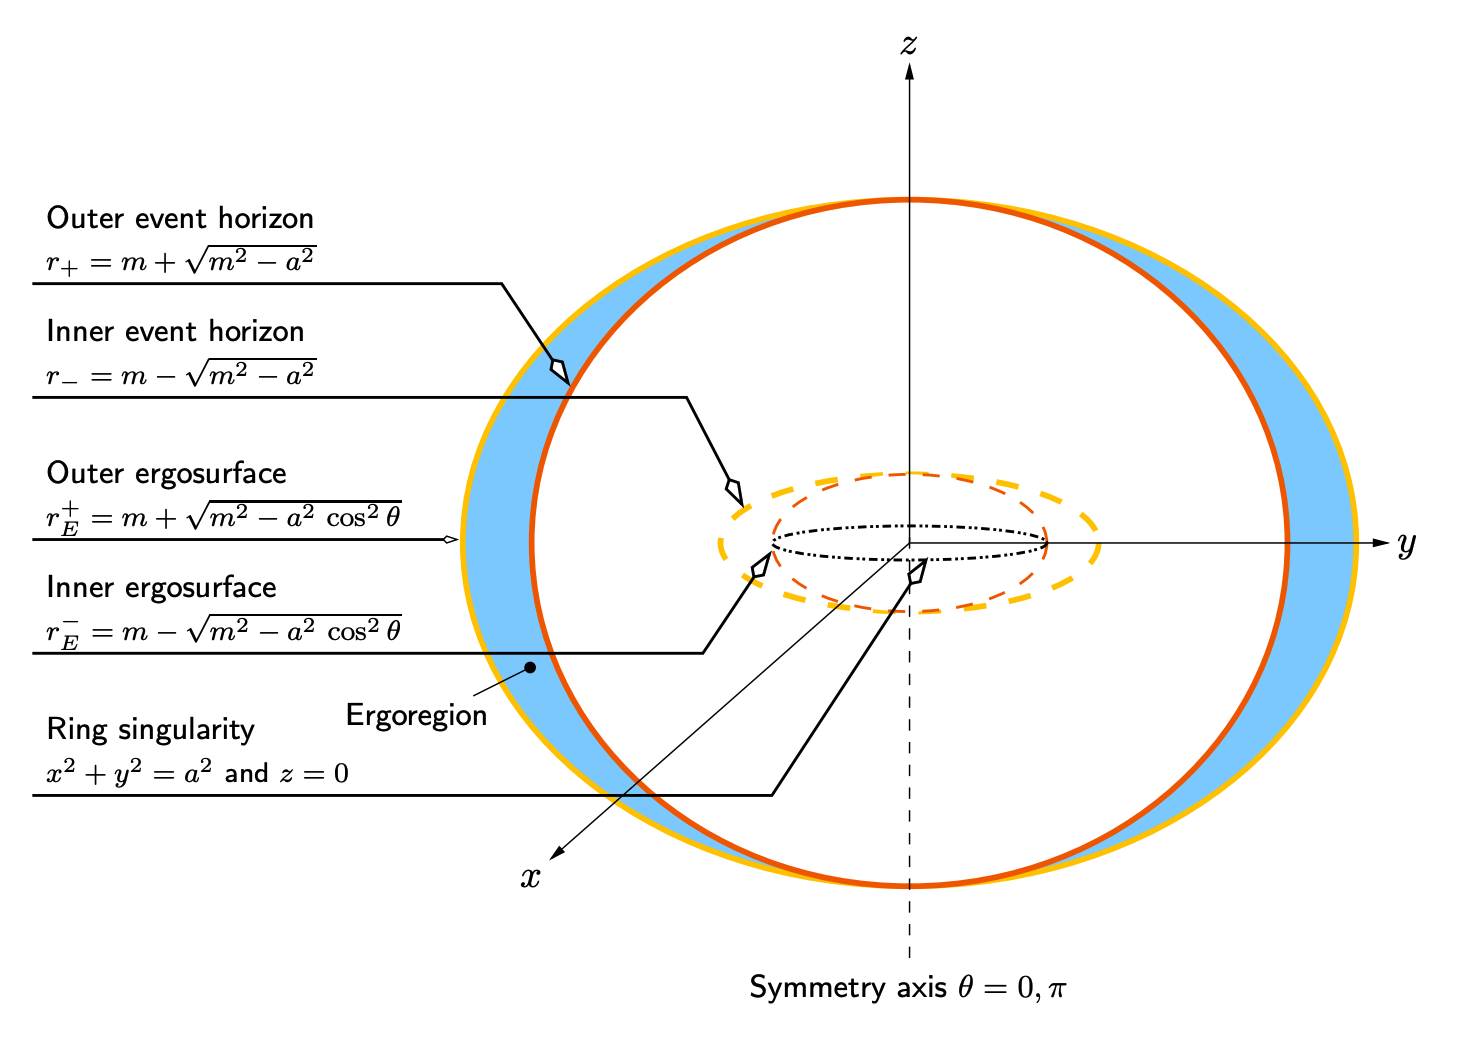
\includegraphics[width=0.8\textwidth]{Kerr Black Hole.png}
    \caption{Schematic Kerr Black Hole~\cite{visser}}
  \end{figure}
\end{frame}
%---------------------------------


%---------------------------------
\begin{frame}{Three Constants}
As always, for a geodesic with affine parameter $\lambda$, we use $x$ to denote the position of the geodesic, just keep in mind that we are working with Boyer-Lindquist coordinates. We use $u$ to denote the velocity vector.
  \begin{block}{Definition}
    The \textit{Lagrangian} is defined as:
    \[
    \mathcal{L}(x, \dot{x}) := \frac{1}{2}g(\dot{x},\dot{x}) = \frac{1}{2}g_{\mu\nu}\dot{x}^\mu\,\dot{x}^\nu.
    \]
    The \textit{conjugate momentum} is given by:
    \[
    p_\mu := \frac{\partial \mathcal{L}}{\partial \dot{x}^\mu} = g_{\mu\nu}\,\dot{x}^\nu.
    \]
  \end{block}
  
  Notice that the physical momentum $p^{\mu}=u^{\mu}$, so lowering the index we have $p_{\mu}=g_{\mu\nu}u^{\nu}$ which is just the conjugate momentum defined above.

\end{frame}

%---------------------------------
\begin{frame}{}
\begin{block}{Lemma}
    $p_t$ and $p_{\phi}$ are constant along the geodesics.
\end{block}
\textit{Pf}:
    Stationary$\implies$ Killing vector $k=(1,0,0,0)$.\\
    Axisymmetric$\implies$ Killing vector $m=(0,0,0,1)$ (wlog, assume it rotates around the z-axis)\\
    So consider how $\xi_{\mu}p^{\mu}$ changes along the geodesic, we can show
    \begin{align}
        p^{\nu}\nabla_{\nu}(\xi_{\mu}p^{\mu})
        &=0
    \end{align}

    
\end{frame}
%---------------------------------


%---------------------------------
\begin{frame}{}
    \begin{itemize}
        \item The energy and angular momentum $E=-k^{\mu}u_{\mu}=-p_t$ and $L=m^{\mu}u_{\mu}=p_{\phi}$ are constant along the geodesic.
        \item  We should not forget there is another trivial invariant $\kappa$ which is the invariant mass of the test particle, defined by 
    \begin{equation}
        \kappa = g_{\mu\nu}u^{\mu}u^{\nu}=g_{\mu\nu}p^{\mu}p^{\nu}
    \end{equation}
    \[
    \kappa \;=\;
    \begin{cases}
    -1 & \text{for timelike geodesics},\\[6pt]
    +1 & \text{for spacelike geodesics},\\[6pt]
    0  & \text{for null geodesics}.
    \end{cases}
    \]
    \end{itemize}
\end{frame}
%---------------------------------





%---------------------------------
\begin{frame}{Hamilton–Jacobi Formalism}
  \begin{block}{Definition}
    The Hamiltonian is defined as:
    \[
    H(x,p) := p_{\mu}\dot{x}^{\mu}-\mathcal{L}(x,\dot{x}) = \frac{1}{2}p_{\mu}g^{\mu\nu}p_{\nu}.
    \]
  \end{block}
  
  \begin{theorem}[Jacobi]
    Let $S(x,\lambda)$ solve the Hamilton--Jacobi equation
    \begin{equation}
        H\!\Bigl(x, \frac{\partial S}{\partial x}\Bigr)
        + \frac{\partial S}{\partial \lambda} = 0
    \end{equation}
    If $x(\lambda)$ satisfies $\dot{x}^{\mu} = \frac{\partial H}{\partial p_{\mu}}\bigl(x, \frac{\partial S}{\partial x}\bigr)$, then $x(\lambda)$ is a geodesic, and along it
    \begin{equation}
        \frac{\partial S}{\partial x^{\mu}} = p_{\mu} \quad \frac{\partial S}{\partial \lambda} = -H
    \end{equation}
\end{theorem}
\end{frame}



\begin{frame}{}
    \begin{itemize}
        \item Since $H$ does not depend explicitly on $\lambda$, $t$, $\phi$, we look for solutions of the form (an ansatz)
    \begin{equation}
        S 
        = 
        -\tfrac{1}{2}\,\kappa\,\lambda
        \;-\;
        E\,t
        \;+\;
        L\,\phi
        \;+\;
        S^{(r\theta)}(r,\theta)
    \end{equation}
    where \(S^{(r\theta)}\) is a function of \(r\) and \(\theta\) to be determined.
    \item We follow the idea of B. Carter~\cite{carter}, we want to find a separable solution, so we further assume $S$ has the following expression
    \begin{equation}
        S \;=\; -\,\tfrac12\,\kappa\,\lambda
        \;-\; E\,t
        \;+\; L\,\phi
        \;+\; S^{(r)}(r)
        \;+\; S^{(\theta)}(\theta)
    \end{equation}
    \end{itemize}
    \begin{definition}
    \[
    Q := p_{\theta}^2 - \cos^2 \theta \left[(\kappa + E^2)a^2 - \frac{L^2}{\sin^2 \theta}\right].
    \]
    \end{definition}
\end{frame}





%---------------------------------
\begin{frame}{The Fourth Constant: Carter Constant}
  \begin{block}{Theorem}
    $Q$ defined above is also constant along geodesics, it is called the Carter constant.
  \end{block}

  \textit{Pf}:
  Substitute the above assumption of $S$ into the H-J equation, multiply by $\Sigma$, rearrange the equation such that the LHS only involves $r$ and the RHS only involves $\theta$:
  \begin{equation}
      \text{LHS}=\Delta\Bigl(\frac{dS^{(r)}}{dr}\Bigr)^2- \kappa r^2
    - \frac{(r^2 + a^2)^2}{\Delta}E^2
    + \frac{4Mra}{\Delta}EL
    - \frac{a^2L^2}{\Delta}
  \end{equation}
  \begin{equation}
      \text{RHS}=-\Bigl(\frac{dS^{(\theta)}}{d\theta}\Bigr)^2
    + \kappa\,a^2\cos^2\theta
    - a^2\sin^2\theta E^2
    - \frac{1}{\sin^2\theta}L^2
  \end{equation}
In order to make the RHS$=-Q$, we add $a^2E^2+L^2$ to both sides, so the equation becomes
\begin{equation}
    \Delta\Bigl(\frac{dS^{(r)}}{dr}\Bigr)^2
    -\kappa r^2
    -\frac{(r^2 + a^2)^2}{\Delta}E^2
    +\frac{4Mra}{\Delta}EL
    -\frac{a^2 L^2}{\Delta} +a^2 E^2 +L^2 = -Q
\end{equation}

\end{frame}

%---------------------------------
\begin{frame}{Geodesic Equations}
\begin{lemma}
We define the functions $R(r)$ and $\Theta(\theta)$ as:
    \begin{equation}
        R(r)=\Delta\Bigl[\kappa r^2-(L - aE)^2-Q\Bigr]
        +\Bigl[E(r^2 + a^2)-La\Bigr]^2
    \end{equation}
    \begin{equation}
        \Theta(\theta)=Q+\cos^2\theta
        \Bigl[(\kappa + E^2)a^2-\frac{L^2}{\sin^2\theta}\Bigr]
    \end{equation}
    Then we have the following two ODEs:
    \begin{equation}
        p_{\theta}^2 \;=\; \bigl(\Sigma\,\dot{\theta}\bigr)^2 \;=\; \Theta(\theta),
        \quad
        p_{r}^2 \;=\; \Bigl(\tfrac{\Sigma}{\Delta}\,\dot{r}\Bigr)^2 \;=\; \tfrac{R(r)}{\Delta^2}
    \end{equation}
\end{lemma}
\textit{Pf}:
$p_{\theta}^2=\Theta(\theta)$ follows immediately after the expression of $Q$. $p_r$ is by the other expression of the Carter constant.
\end{frame}

\begin{frame}{}
    \begin{theorem}
        The geodesics of a test particle around the Kerr black hole can be expressed as:
        \begin{equation}
            \dot{\theta} = \pm\,\frac{1}{\Sigma}\,\sqrt{\Theta},
        \quad\quad
        \dot{r} = \pm\,\frac{1}{\Sigma}\,\sqrt{R}
        \end{equation}
        \begin{equation}
            \dot{\phi} = -\frac{1}{\Sigma}(a E-\frac{L}{\sin^2\theta})+\frac{a}{\Delta\Sigma}[E(r^2+a^2)-aL]
        \end{equation}
        \begin{equation}
            \dot{t} = -\frac{1}{\Sigma}(a^2 E \sin^2\theta-aL) + \frac{r^2+a^2}{\Delta\Sigma}[E(r^2+a^2)-aL]
        \end{equation}
    \end{theorem}
    \textit{Pf}:
    $\dot{\theta}$ and $\dot{r}$ follow from the above lemma. The other two can be shown by solving \begin{equation}
        \begin{cases}
            p_t = g_{tt}\dot{t} +g_{t\phi}\dot{\phi} = -E \\
            p_\phi = g_{\phi t}\dot{t} + g_{\phi\phi}\dot{\phi} = L
        \end{cases}
    \end{equation}
\end{frame}

%---------------------------------
\begin{frame}{Numerical Method}
  \begin{itemize}
    \item Mino time $d\lambda = \Sigma\, d\sigma$~\cite{mino} decouples the motion:
    \[
    \Bigl(\frac{dr}{d\sigma}\Bigr)^2 = R(r), \qquad \Bigl(\frac{d\theta}{d\sigma}\Bigr)^2 = \Theta(\theta)
    \]
    \item We integrate the derivatives, smooth at turning points:
    \[
    \frac{d^2r}{d\sigma^2} = \tfrac{1}{2}R'(r), \qquad \frac{d^2\theta}{d\sigma^2} = \tfrac{1}{2}\Theta'(\theta)
    \]
    together with $d\phi/d\sigma$, $dt/d\sigma$ from the theorem above.
    \item An orbit is chosen by its turning points $r_{\mathrm{p}}, r_{\mathrm{a}}$ and inclination $\iota$: Newton's method solves $R(r_{\mathrm{p}}) = R(r_{\mathrm{a}}) = 0$ for $E$, $L$, $Q$.
    \item Adaptive Dormand--Prince Runge--Kutta~\cite{hairer}; first integrals hold to $10^{-9}$; matches Hamilton's equations to $3\times 10^{-9}$.
  \end{itemize}
\end{frame}

\begin{frame}{Example: $a = 0.9$, $r_{\mathrm{p}} = 6$, $r_{\mathrm{a}} = 12$, $\iota = 45^\circ$}
  \begin{figure}
    \centering
    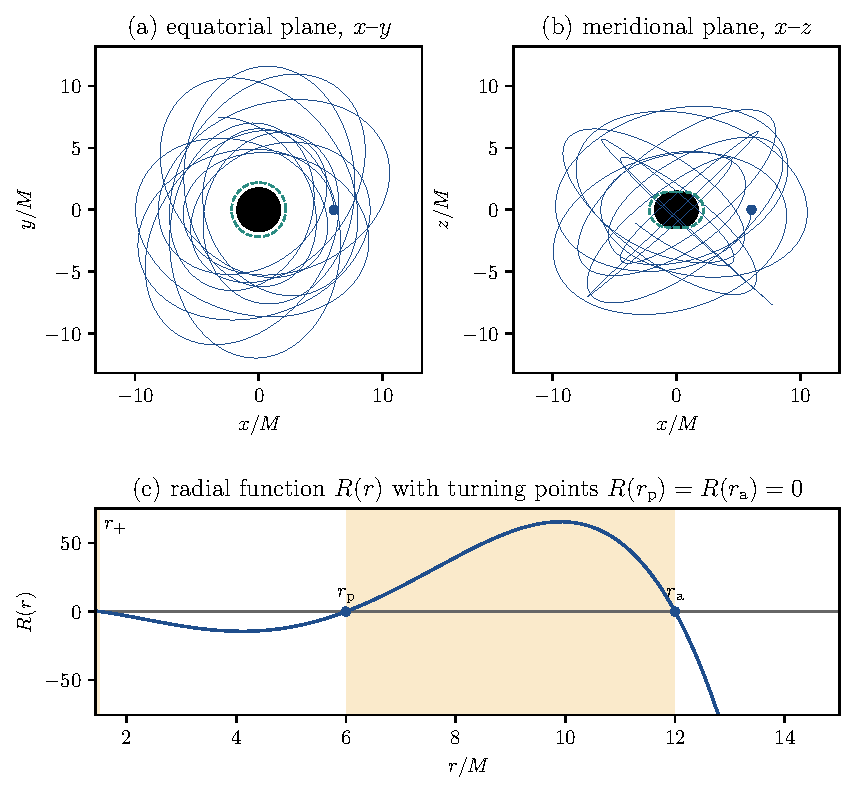
\includegraphics[height=0.70\textheight]{kerr_orbit.pdf}
  \end{figure}
  \vspace{-0.6em}
  {\small Periapsis advance plus Lense--Thirring precession of the orbital plane. Interactive version: \texttt{kerr\_geodesics.html}.}
\end{frame}

%---------------------------------
\begin{frame}{Extension to Charged Particle Dynamics}
  \begin{itemize}
    \item Charged particle in a stationary, axisymmetric dipole magnetic field $A_{\mu}(r,\theta)$ on a fixed Kerr background~\cite{takahashi}:
    \[
    H = \tfrac{1}{2}g^{\mu\nu}(\pi_{\mu} - qA_{\mu})(\pi_{\nu} - qA_{\nu})
    \]
    \item $t$ and $\phi$ are still cyclic, so $E$, $L$ and $\kappa$ are still conserved.
    \item But $A_{\mu}$ couples $r$ and $\theta$: the Hamilton--Jacobi equation no longer separates, there is no Carter-type fourth constant, and the poloidal motion can be chaotic.
    \item Orbits combine gyration around field lines, bouncing along them, and toroidal drift; the next slide shows two trajectories for \(a=0.9M\) that differ only in the injection angle.
  \end{itemize}
\end{frame}


\begin{frame}{}
      \begin{figure}[H]
    \centering
    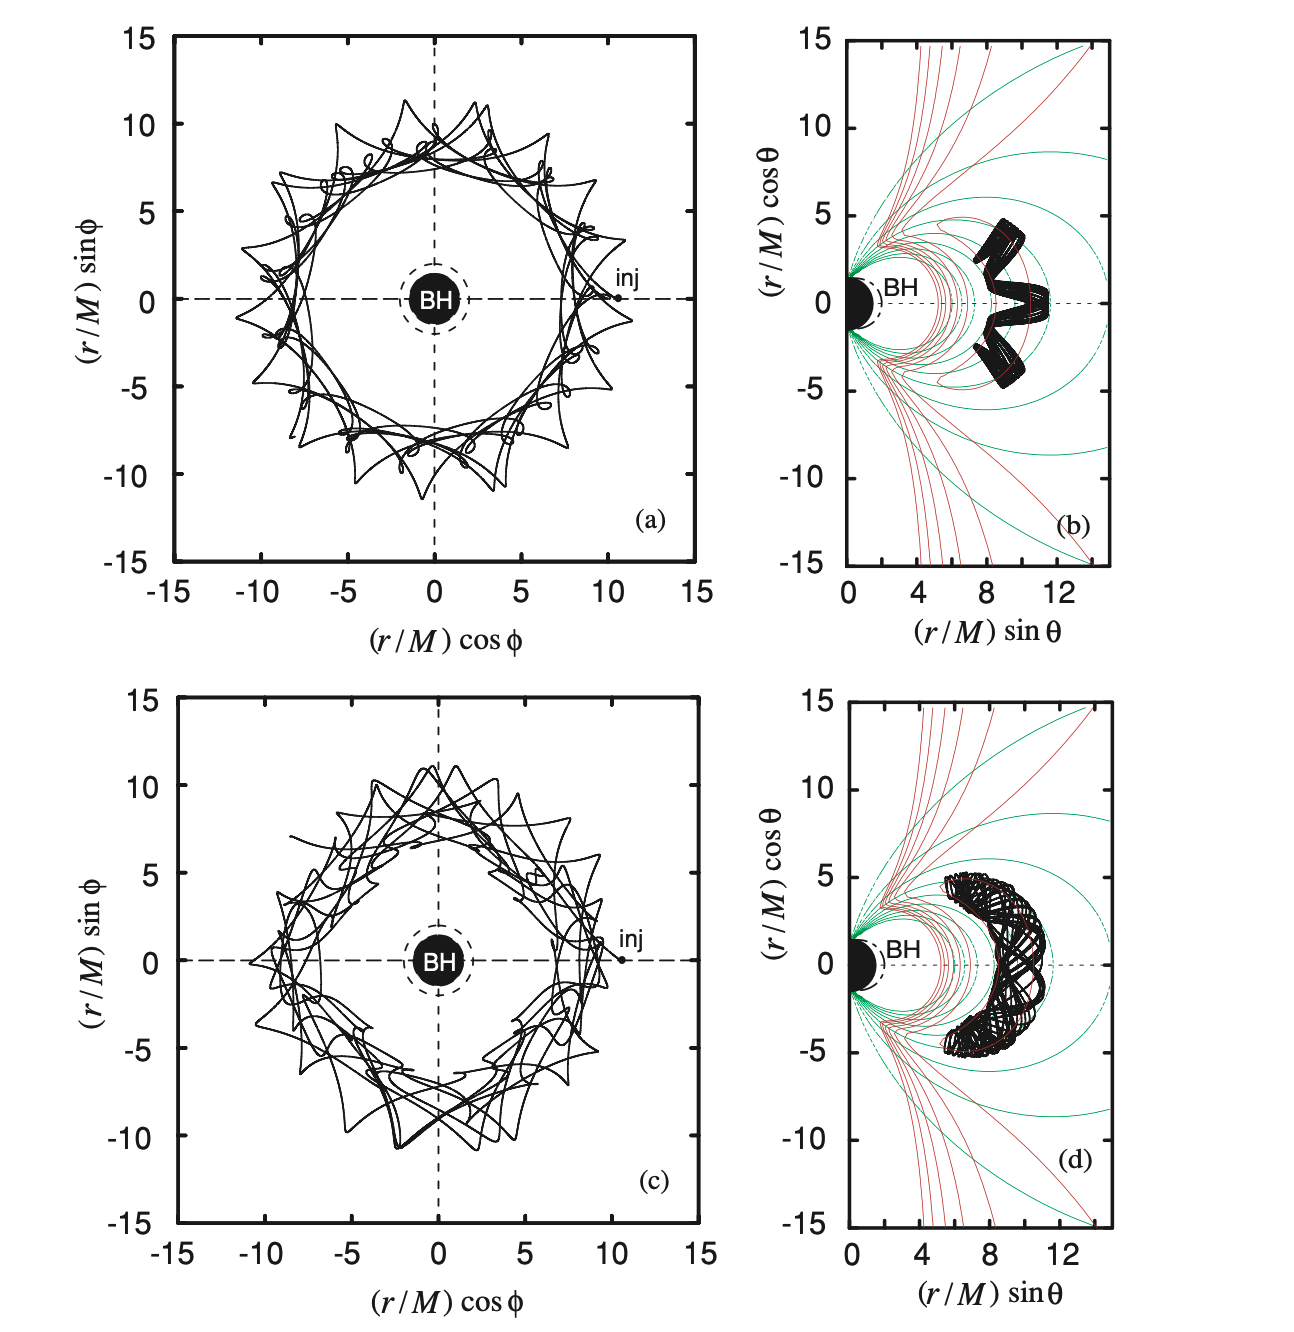
\includegraphics[width=0.6\textwidth]{geodesic2.png}
    \caption{Reproduced from Fig.~6 of~\cite{takahashi}}
  \end{figure}
\end{frame}


%---------------------------------
\begin{frame}{References}
  \footnotesize
  \begin{thebibliography}{9}
    \bibitem{oneill}
      B.~O'Neill, 
      \emph{The Geometry of Kerr Black Holes},
      A K Peters/CRC Press, 1995.
    \bibitem{schutz}
      B.~Schutz,
      \emph{A First Course in General Relativity},
      2nd ed., Cambridge University Press, 2009.
    \bibitem{wald}
      R.~M.~Wald,
      \emph{General Relativity},
      The University of Chicago Press, 1984.
    \bibitem{visser}
      M.~Visser,
      \emph{The Kerr Spacetime: A Brief Introduction},
      arXiv:0706.0622 [gr-qc], 2007.
    \bibitem{carter}
      B.~Carter,
      \emph{Global Structure of the Kerr Family of Gravitational Fields},
      Phys. Rev. \textbf{174}, 1559 (1968).
    \bibitem{goldstein}
      H.~Goldstein,
      \emph{Classical Mechanics}, 3rd ed.,
      Addison Wesley, 2001, Chapter 10.
    \bibitem{mino}
      Y.~Mino,
      \emph{Perturbative approach to an orbital evolution around a supermassive black hole},
      Phys. Rev. D \textbf{67}, 084027 (2003).
    \bibitem{hairer}
      E.~Hairer, S.~P.~N{\o}rsett and G.~Wanner,
      \emph{Solving Ordinary Differential Equations I: Nonstiff Problems}, 2nd ed., Springer, 1993.
    \bibitem{takahashi}
      M.~Takahashi and H.~Koyama,
      \emph{Chaotic motion of Charged Particles in an Electromagnetic Field Surrounding a Rotating Black Hole},
      arXiv:0807.0277v1 [astro-ph], 2008.
  \end{thebibliography}
\end{frame}

\end{document}
